\chapter{Conclusion, discussion and prospect}
\begin{comment}
The Belle II experiment is built upon the success of its predecessor Belle and many other great efforts of exploring the mysteries of flavor physics, which have expand our knowledge and understanding of elementary particle physics. One of the most outstanding outcome of these efforts is the Standard Model, which it's capable of well describing a variety of experimental results in a large energy scale and fine precision for the past few decades. And yet open questions that still draws attention from particle physicists remain, wait to be discovered as New Physics. One of the most important question is that why the universe is mass-dominated while anti-matter seems to be vanished. 

Belle II is aimed to search for New Physics through the precise measurements of related topics in heavy flavor physics at the world-record luminosity frontier. SuperKEKB accelerator is designed with asymmetric beam
energies to provide a boost to the center-of-mass system and thereby allow for time-dependent
\textit{CP} symmetry violation measurements. The products of collision is in a very clean environment, with 40 times higher luminosity of peak at Belle. This create excellent opportunities for physicists to look for the undiscovered source of \textit{CP} violation, for which the existing explanation from the complex phase of CKM matrix can't described the observed level of asymmetry in our universe.

$b\to s$ transition is an important flavor coupling process to be examined in search for New Physics. The \textit{CP} violation in such process was first observed after the precise measurement in $b\to c$ with a small tension. So far the precision of the measurement of $\it{CP}$ parameter $\mathcal{S}$ in $b\to s$ is still in an arguable difference with tree-level process considering the existing uncertainty, which allows a decent margin for New Physics. The representative processes of $b\to s$ are resonant decay such as $B^0 \to \eta^{'} K_S^0$, $B^0 \to \phi K_S^0$ and decay like $B^0 \to K_S^0  K_S^0  K_S^0$, on which Belle II experiment will have an excellent prospective sensitivity.

This thesis presents the first attempt to study the time-dependent $\it{CP}$ violation in $B^0 \to K_S^0  K_S^0  K_S^0$ using early phase 3 data of Belle II and latest MC sample. In order to reconstruct clean signal sample of $B^0$ , $K_S^0$ reconstruction performance is critical because of the unique characteristics of this decay. A KsFinder based on FastBDT classification algorithm is developed to offer a goodness indicator of traditional cut-based reconstruction of $K_S^0$. The performance of this new KsFinder is validated to have a great background rejection power at  with small signal loss in the maximum FOM case. $B^0$ are reconstructed with a good significance even with very low statistics with a good agreement with MC prediction and Belle experience.
The overall efficiency of $B^0$ is slightly improved than Belle with slightly higher beam background condition in current Belle II. The measurement  of the \textit{CP} fit is conducted based on the reconstruction. The $\it{CP}$ fit using artificial model containing resolution functions from different sources are built with precise study of MC signal samples and the data sideband . As for flavor tagging information, wrong fraction as mandatory parameters in signal $\Delta t$ distribution, are implemented too. The coefficient of signal and background in the $\it{CP}$ fit model is determined by the signal extraction 2D fit over $M_{bc}$ and $\Delta E$. For each event, the signal fraction is calculated based on the $M_{bc}$ and $\Delta E$ using the 2D fit model, which is used as a discrete observable in $\it{CP}$ fit model.
\end{comment}

 
 
 
\begin{comment}
Furthermore, the key to improve the precision of this measurement highly depends on the better signal reconstruction efficiency and vertex fitting. Both of these performances have been primarily studied to be either same competitive or outperformed with current Belle II condition compared to Belle. $K_S^0$ finder which guarantees the signal efficiency in the key role can be optimized by taking a better correction from data MC comparison in future. Besides, other algorithm such as deep neural network (DNN) may give a better discrimination but haven't been studied yet. One of the major concern is that tracking efficiency of $K_S^0$ is degraded by their long flight length, and it damages the advantage of having a larger detector volume in Belle II design motives. The expected boost in $K_S^0$ reconstruction is about 15\% which yields nearly 50\% more $B^0$ in this channel. Due to this issue, even with improved reconstruction strategies, the efficiency is not largely boosted as expected. This degradation may become even worse when higher background level is induced in future operation, the related improvement both from hardware and software is under construction. Thanks to extra PXD layers in Belle II, decay vertex now have a better constraint and smaller uncertainties. The resolution studies on \textit{CP} and tag side shows a clear improvement on vertexing accuracy. The vertex reconstruction still has a margin to improve after the full installation of PXD layer 2. The modeling of resolution function should also evolve with better understanding of vertexing performance along with data collection. The analysis presented in this thesis, including various strategies and supporting studies, paves a solid way for the time-dependent \textit{CP} violation measurement with Belle II data in the next few years. 
\end{comment}

The $\it{CP}$ parameters measurement is performed based on the validation of analysis strategies by blind analysis.  
The blind fit is performed which shows a consistent fit result for $\it{CP}$ parameters compared to the simulation input. The linearity and pull of the $\it{CP}$ fit are checked to validate the reliability of the fit procedures. The fit result on $B^0$ lifetime using experiment data is also agreed with the current value in PDG with a relatively large statistical uncertainty due to the low statistics from data.

After the $\it{CP}$ fit procedures are validated, the permission of $\it{CP}$ fit using data is given by the Belle II collaboration, the $\it{CP}$ parameters $\mathcal{S}$ and $\mathcal{A}$ using Belle II early data in 2019 and 2020 spring and summer is performed. The result is shown in Equation \ref{eq:data_fit_cp}.

\begin{equation}\label{eq:data_fit_cp}
\begin{split}
\mathcal{S}=- sin(2\phi_1) & = -0.82 \pm 0.85(\text{stat}) \pm 0.07(\text{syst}) \\
\mathcal{A} & = -0.21\pm 0.28(\text{stat}) \pm 0.06(\text{syst})\\
\end{split}
\end{equation}  

The result agrees with the prediction of the Standard Model and the previous results from Belle and BaBar. The systematics study is performed considering the main contributing sources at the moment. The $\it{CP}$ parameters precision from this study is majorly limited due to the large statistical uncertainties from very low statistics, which leads to no clear evidence or hint on the NP effects. 
 
What is worth of noticing is that main analysis tools required by performing the $\it{CP}$ measurement on this channel are in a good stage of the development. The newly developed \textit{KsFinder} contributes much in improving the signal significance by effectively rejecting fake $K_S^0$, which is also useful in background rejection for other channels with $K_S^0$ in the final state.  The model of the resolution of vertex positions has been studied using MC sample and sideband data, which is benefiting from the understanding of vertex reconstruction performance in the current Belle II detectors. To make a proper use of the reconstructed vertex information and perform $\it{CP}$ fit compactly, a new $\it{CP}$ fitter is built and being validated, which will serve as a multi-functional analysis tool for Belle II $\it{CP}$ violation study in future. 
 
 %The Belle II experiment is crucial in these channels because of the cleaner background environment and better sensitivity compared with LHCb.

\subsection{Improvements in statistical uncertainty}
This study has shown a good potential of performing $\it{CP}$ measurement in Belle II for the incoming years with more and more data recorded. The precision on $\mathcal{S}$ requires the large luminosity as shown in Figure \ref{fig:sensitivity} and the statistical uncertainty in this thesis fits in the scale. With 50 $ab^{-1}$ luminosity from the full Belle II data sample in future, the statistical uncertainty is expected to be reduced. The $\it{CP}$ fit on the MC sample with different mount of events used reflects that the statistical uncertainty is reduced proportionally around factor of $\frac{1}{\sqrt{N}}$, where $N$ is the events used in $\it{CP}$ fit. Therefore, the expected reduction of statistical uncertainty due to increased data sample with current reconstruction efficiency is predicted as Figure \ref{fig:stats_future}. The projected statistical uncertainty is slight reduced compared with the Belle result at 1 ab$^{-1}$. In future Belle II with full data sample, the estimated statistical uncertainty is about 0.0302 as shown in Figure \ref{fig:stats_future}, which is also improved compared to the original estimation at 0.037 from Belle II technical design report in Table \ref{tab:sensitivity}. From Table \ref{tab:b0stats}, the current $B^0$ reconstruction efficiency is about 35\% which could be further optimized mainly by improving $K_S^0$ efficiency from the current CDC-only tracking. Due to the enlarged VXD volume of Belle II, the expected $K_S^0$ acceptance region is larger than Belle, which could contribute more on $B^0$ signal yield in future to help reduce the statistical uncertainty. 

\begin{figure}[htpb]
\centering
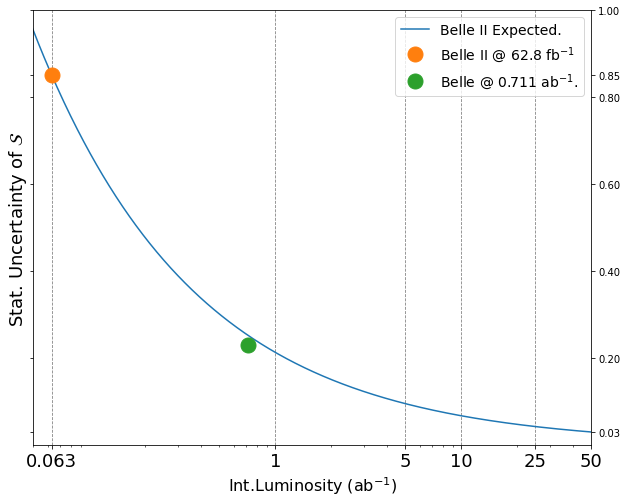
\includegraphics[width=0.6\linewidth]{stats_b2}
\caption{Statistical uncertainty of $\mathcal{S}$ extrapolation based on the current result of $B^0 \to K_S^0  K_S^0  K_S^0$ in Belle II.}
\label{fig:stats_future}
\end{figure}




 Along with the data collection continues, we will be able to finely test and improve the analysis strategies and tools to a better stage using data, such as improving the reconstruction efficiency and purity of $B^0$ when the luminosity ramps up to much higher level with much higher backgrounds. At integral luminosity at 50 ab$^{-1}$ level, the statistical uncertainty of this decay on $\Delta \mathcal{S}$ would be trimmed down to a comparable value around $0.03$ which is close the Standard Model correction, offering a much better probe on whether New Physics is influential at this level of precision. The progress that has been made so far in this thesis paves a well-constructed and solid path towards future results.
 From the current result, the chance of having a much precised measurement in the next a few years on this channel is very promising and searching New Physics effect in penguin-mode $b\to s$ transition from Belle II is proven to be an exciting and important topic. 
 
 

